\subsection{SMART objective Justification}
\label{app:smartobj}
This section expands on the objectives listed in the “Technical objectives” section. It specifies the SMART (Specific, Measurable, Achievable, Relevant, and Time-bound) nature of the objectives.


\textbf{Objective 1: Implement real time localisation and mapping capability}

\bgroup
\rowcolors{2}{gray!15}{white}
\begin{tabularx}{\textwidth}{M{1cm}|R{14cm}}
    \textbf{S} & Implement the ability to localise the robot’s position within the 3D point cloud generated by the LiDAR sensor.\\
    \textbf{M} & This capability will be complete when the map produced by the LiDAR sensor correctly resembles the testing environment. A 2D overlay image of the map can be analysed to the known testing environment map to address accuracy and completeness. \\
    \textbf{A} & This capability is commonly achieved in robotics by utilising a SLAM algorithm, these algorithms are heavily supported and documented within ROS. \\
    \textbf{R} & For the robot to autonomously navigate its way through the cave environment, it must be able to recognise its position within the cave point cloud map. \\
    \textbf{T} & This is a key capability that will allow for autonomous behaviour to be built on top of, hence it is aimed to be completed by June 18\textsuperscript{th}. This objective however can still be completed in parallel with the other technical objectives in an agile approach
\end{tabularx}\\


\textbf{Objective 2: Design, Implement \& Optimise a Pathfinding Algorithm}

\begin{tabularx}{\textwidth}{M{1cm}|R{14cm}}
    \textbf{S} & Implement an algorithm which can generate an ideal path based on LiDAR data, recent movement, and generated way points.\\
    \textbf{M} & Objective is completed when the robot can successfully plan paths fully autonomously (no prior instruction) and semi-autonomously (between pre-defined waypoints). \\
    \textbf{A} & This is achievable as there is a wealth of information on the internet regarding robotics control algorithms using LiDAR. Pathfinding algorithms already exist and can, therefore, form a basis for the robot’s system. \\
    \textbf{R} & For the robot’s autonomous control algorithms to work, they require input from a pathfinding algorithm. \\
    \textbf{T} & Implementing autonomy to the robot is the overarching goal of this year’s iteration of the CaveX project. However, testing will be required therefore, this objective should be completed with time left to conduct testing. Hence, it should be completed by September 10\textsuperscript{th}.
\end{tabularx}\\

\newpage
\textbf{Objective 3: Implement terrain sensing and gait control system}

\begin{tabularx}{\textwidth}{M{1cm}|R{14cm}}
    \textbf{S} & Implement hardware and software which can sense the surface characteristics beneath each foot and adjust the gait of each leg accordingly.\\
    \textbf{M} & Objective is completed when the robot’s speed or stability, which can be measured using optical tracking, is improved using motor feedback or force sensing resistors. \\
    \textbf{A} & This is achievable as an iterative test-based approach will allow for the development of a system which can account for ground characteristics. \\
    \textbf{R} & To increase the robot’s ability to traverse cave structures, it should adjust its gait according to the variety of surfaces it will traverse. \\
    \textbf{T} & Ideally, this objective should be complete before OB2 to allow for optimal performance, the target date for completion is 13\textsuperscript{th} August. OB2 does not directly depend on this objective meaning agile development is conserved. \\
\end{tabularx}

\textbf{Objective 4: Implement obstacle detection and avoidance capability}

\begin{tabularx}{\textwidth}{M{1cm}|R{14cm}}
    \textbf{S} & Detect obstacles using peripheral sensors \& adjust the robot’s path to avoid them. \\
    \textbf{M} & The robot can be tested with obstacles to determine if the path planning algorithm takes obstacles into consideration. The object is complete when the robot demonstrates its ability to avoid obstacles. \\
    \textbf{A} & This objective is achievable as it is a problem in robotics which has been solved using a variety of different methods. There is a range of literature for using data from a LiDAR scanner in ROS to detect and avoid obstacles. \\
    \textbf{R} & Obstacle detection and avoidance is a very important aspect of autonomous systems. Without obstacle avoidance the robot risks failing to effectively search a large cave area and potential collisions with undetected obstacles may cause damage to the robot’s hardware.\\
    \textbf{T} & This objective is planned to be completed by 10\textsuperscript{th} Sept. A precursor to obstacle avoidance is having a successful path planning algorithm in place which is outlined in objective 2, however the obstacle detection software can be done independently.\\   
\end{tabularx}

\textbf{Objective 5: Implement Real-time Monitoring System}

\begin{tabularx}{\textwidth}{M{1cm}|R{14cm}}
    \textbf{S} & Implement a convenient interface for the user to send commands to the robot and receive sensor data remotely in real time. \\
    \textbf{M} & Objective is completed when the robot can continuously send its state wirelessly to and receive commands from another device. \\
    \textbf{A} & This is achievable as pre-made software exists for wireless communication with ROS-based robots and software can be written for communication via the internet. \\
    \textbf{R} & For operators to ensure the robot is functioning correctly and for efficient software development, real-time two-way communication with the robot is necessary. \\
    \textbf{T} & This objective has a completion date by 16\textsuperscript{th} July. If this objective is completed early, it will significantly help the team with testing and debugging. \\
\end{tabularx}
\egroup

\newpage
\subsection{Stakeholder Analysis}
\label{app:stakeholder}

\begin{figure}[H]
        \centering
        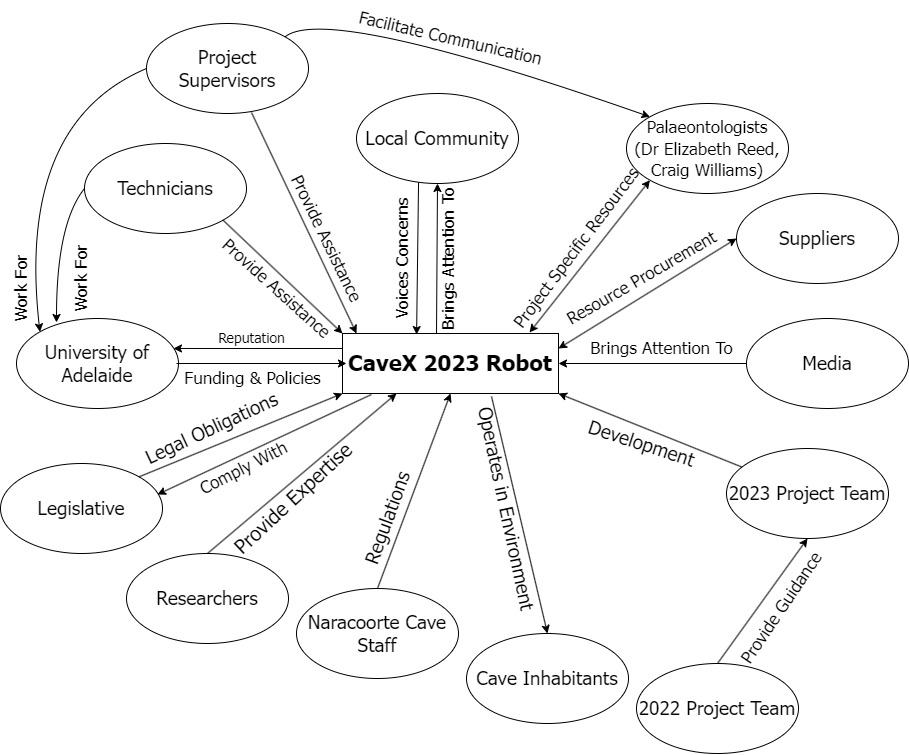
\includegraphics[scale = 0.42]{StakeholderMap_CaveX.jpg}
        \caption{Stakeholder map showing interactions between the project and those that have influence, or are influenced by the project.}
\end{figure}

\begin{figure}[H]
        \centering
        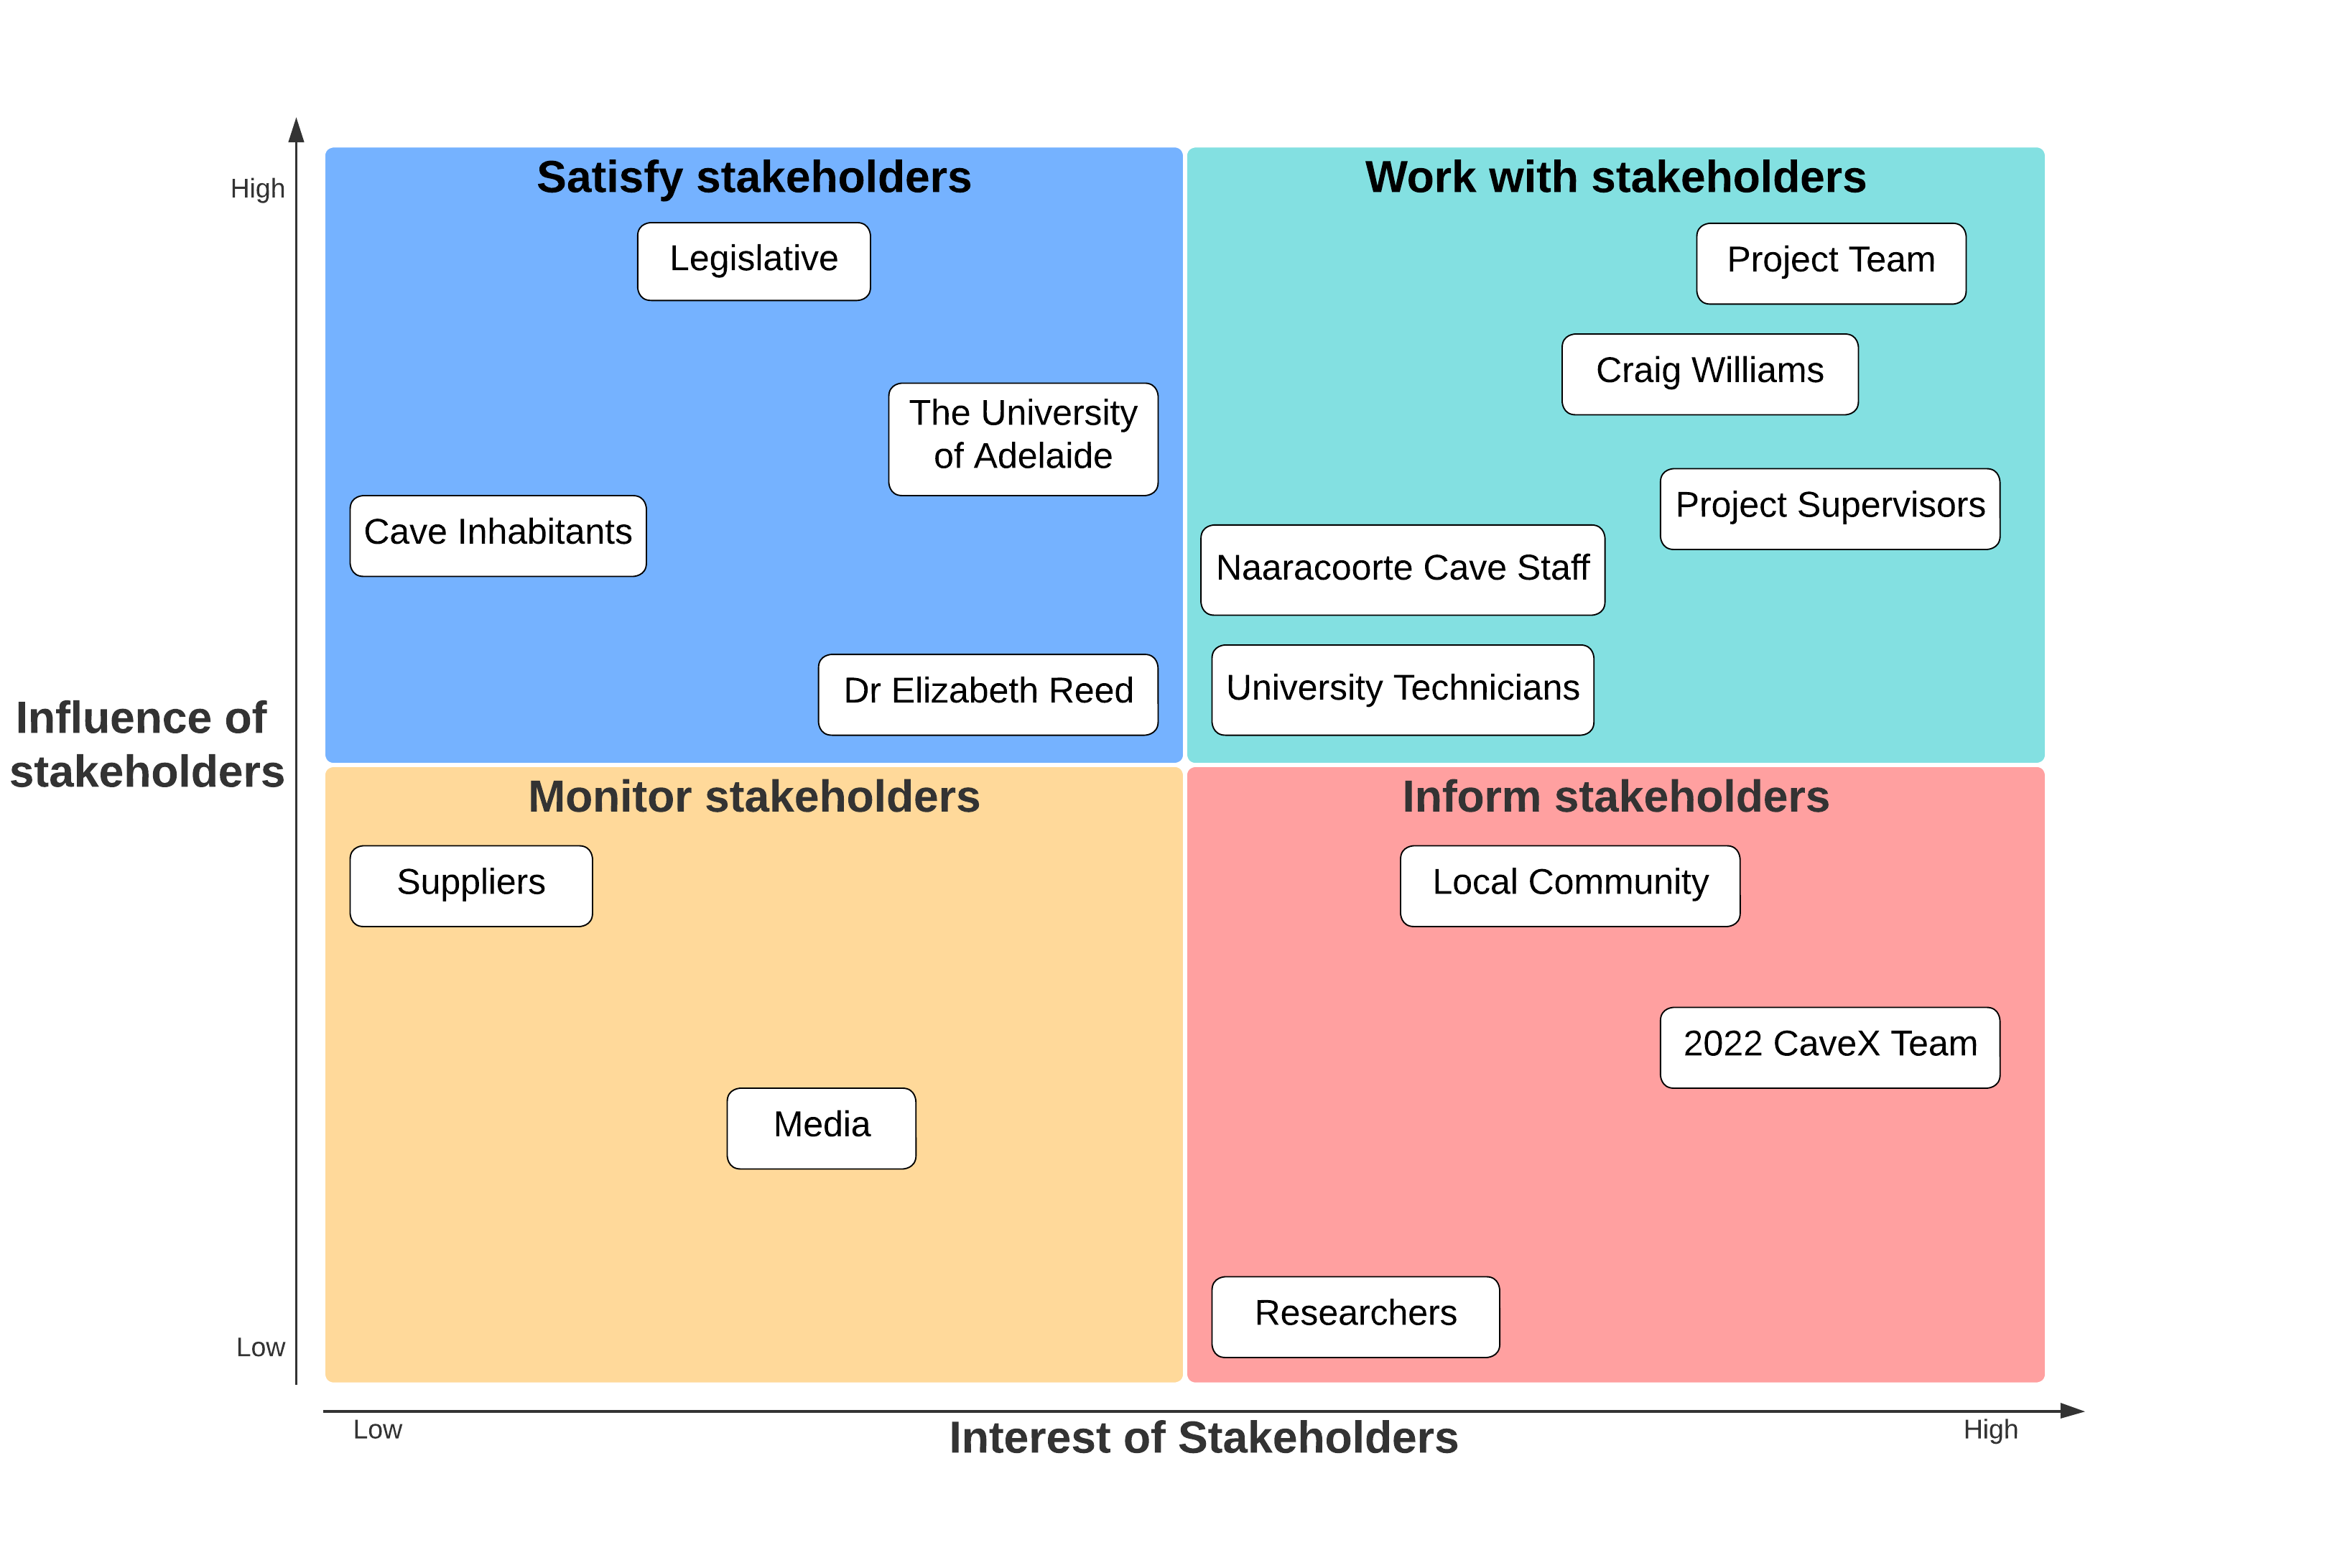
\includegraphics[scale = 0.5]{Stakeholder Influence-Interest Map.png}
        \caption{Influence and interest grid of various stakeholders}
\end{figure}

\newpage
\subsection{Scenario Based Needs Analysis}
\label{app:scenario-based-needs-analysis}

\begin{figure}[H]
        \centering
        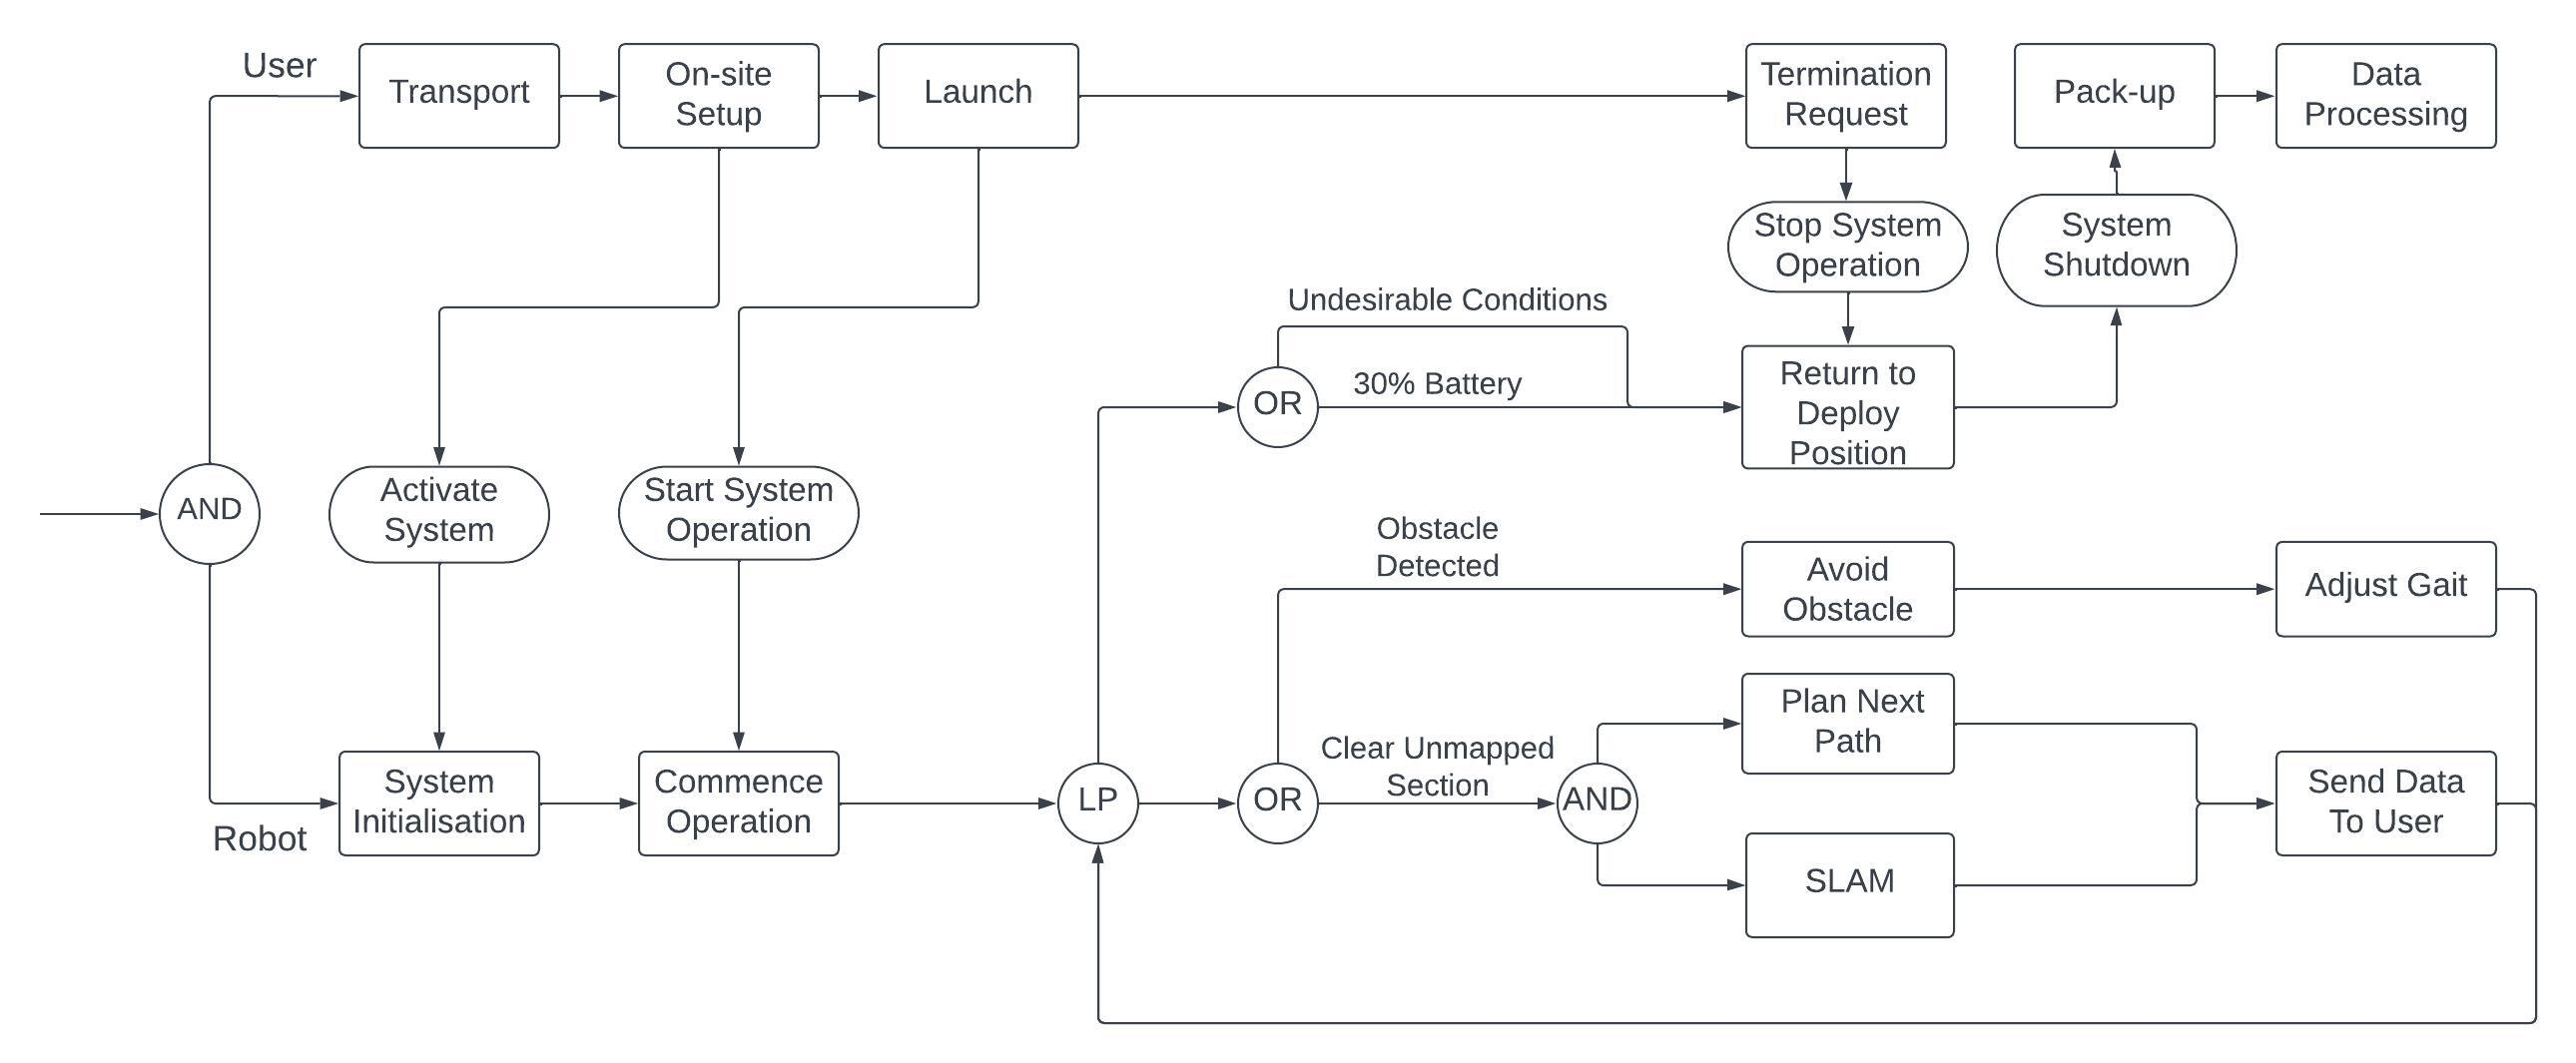
\includegraphics[scale = 0.55,angle=90]{FFBD.jpeg}
        \caption{Scenario-based User Needs Analysis}
        \label{fig:FFBD}
\end{figure}

\newpage
\subsection{System Context Diagram}
\begin{figure}[H]
    \centering
    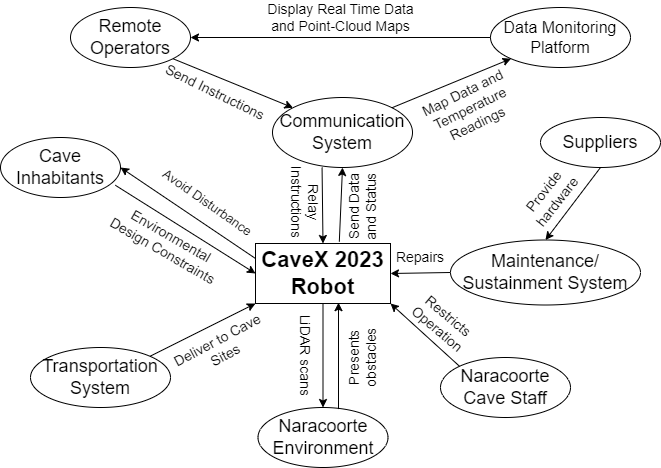
\includegraphics[scale=0.5]{images/system_context.drawio.png}
    \caption{System context diagram displaying interfaces with key external entities}
    \label{fig:system_context}
\end{figure}

\newpage
\subsection{CaveX 2021 Stakeholder Needs}
\label{app:stakeholderNeeds}
\begin{figure}[H]
        \centering
        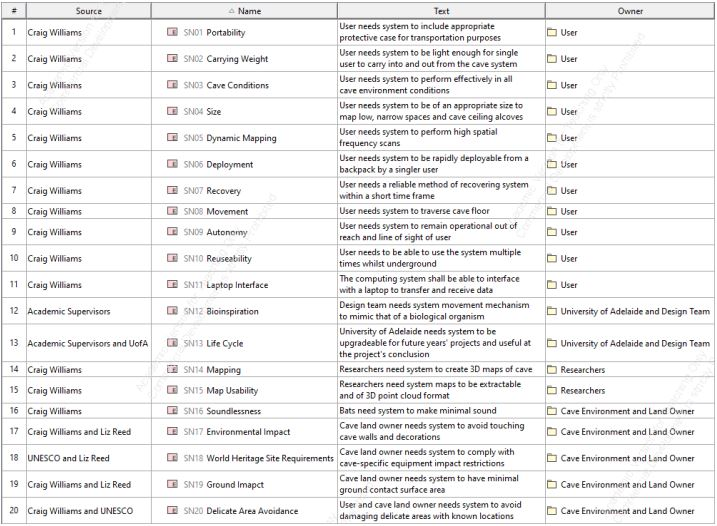
\includegraphics[scale = 1.1, angle=90]{SN_2021.JPG}
        \caption{CaveX Stakeholder Needs Table - Needs gathered from stakeholder interviews and
environmental constraints (Cooper et al. 2021).}
        \label{fig:stakeholderNeeds}
\end{figure}

\newpage
\subsection{CaveX 2021 System Requirements}
\label{app:systemRequirements}
\begin{figure}[H]
        \centering
        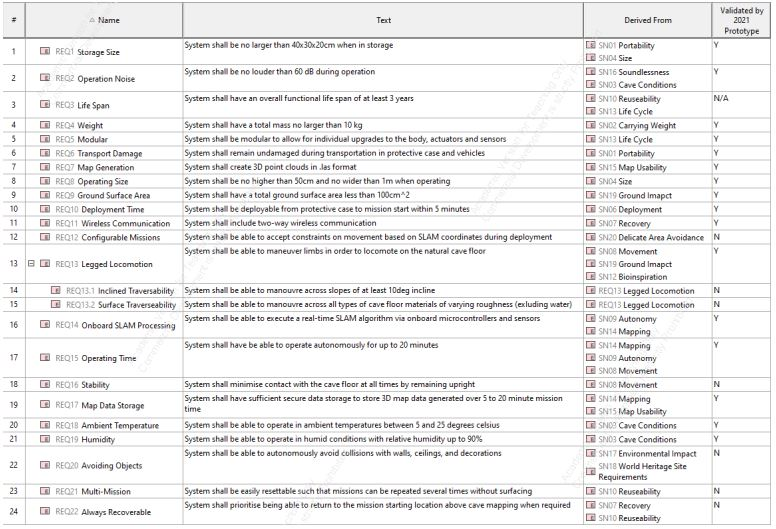
\includegraphics[scale = 1.05, angle=90]{2021SysReq.JPG}
        \caption{CaveX System Requirements Table - Requirements with ID, Description, derivation
from stakeholder needs and applicable traceability (Cooper et al. 2021).}
        \label{fig:systemRequirements}
\end{figure}

\newpage
\subsection{CaveX 2023 User Needs}
\label{app:2023userneeds}
\rowcolors{2}{gray!25}{white}
\begin{xltabular}{\textwidth}{M{2cm}M{6cm}M{4cm}M{2cm}}
    \caption{CaveX 2023 User Needs.}\label{tab:userneeds} \\ \hline
    \rowcolor{gray!50}
    \textbf{Identifier} & \textbf{Description} & \textbf{Traceability} & \textbf{Criticality}
    \\ \hline
    \csvreader[late after line = \\, separator = semicolon]{./csv/2023_CaveX__UserNeeds.csv}{1 = \a, 2 = \b, 3 = \c, 4 = \d}{\a & \b & \c & \expandafter\cellcolor\expandafter{\romannumeral`\^^@\csvcoliv}\csvcoliv}
    \hline
\end{xltabular}

\newpage
\subsection{CaveX 2023 System Requirements}
\label{app:2023sysreqs}
\bgroup
\rowcolors{2}{white}{gray!25}
\begin{xltabular}{\textwidth}{M{1.7cm}M{3cm}M{2.1cm}M{2.4cm}M{2cm}M{2.4cm}}
    \caption{CaveX 2023 System Requirements.}\label{tab:sysreq} \\ \hline
    \rowcolor{gray!50}
    \textbf{Identifier} & \textbf{Description} & \textbf{Traceability} & \textbf{Functionality} & \textbf{Criticality} & \textbf{Verification Method}
    \\ \hline
    \csvreader[late after line = \\, separator = semicolon]{./csv/2023_CaveX__SystemRequirements.csv}{1 = \a, 2 = \b, 3 = \c , 4 = \d, 5 = \e, 6 = \f}{\a & \b & \c & \d & \expandafter\cellcolor\expandafter{\romannumeral`\^^@\csvcolv}\csvcolv &\f}
    \hline
\end{xltabular}
\egroup

\newpage
\subsection{Work Breakdown Structure}
\label{app:WBS}
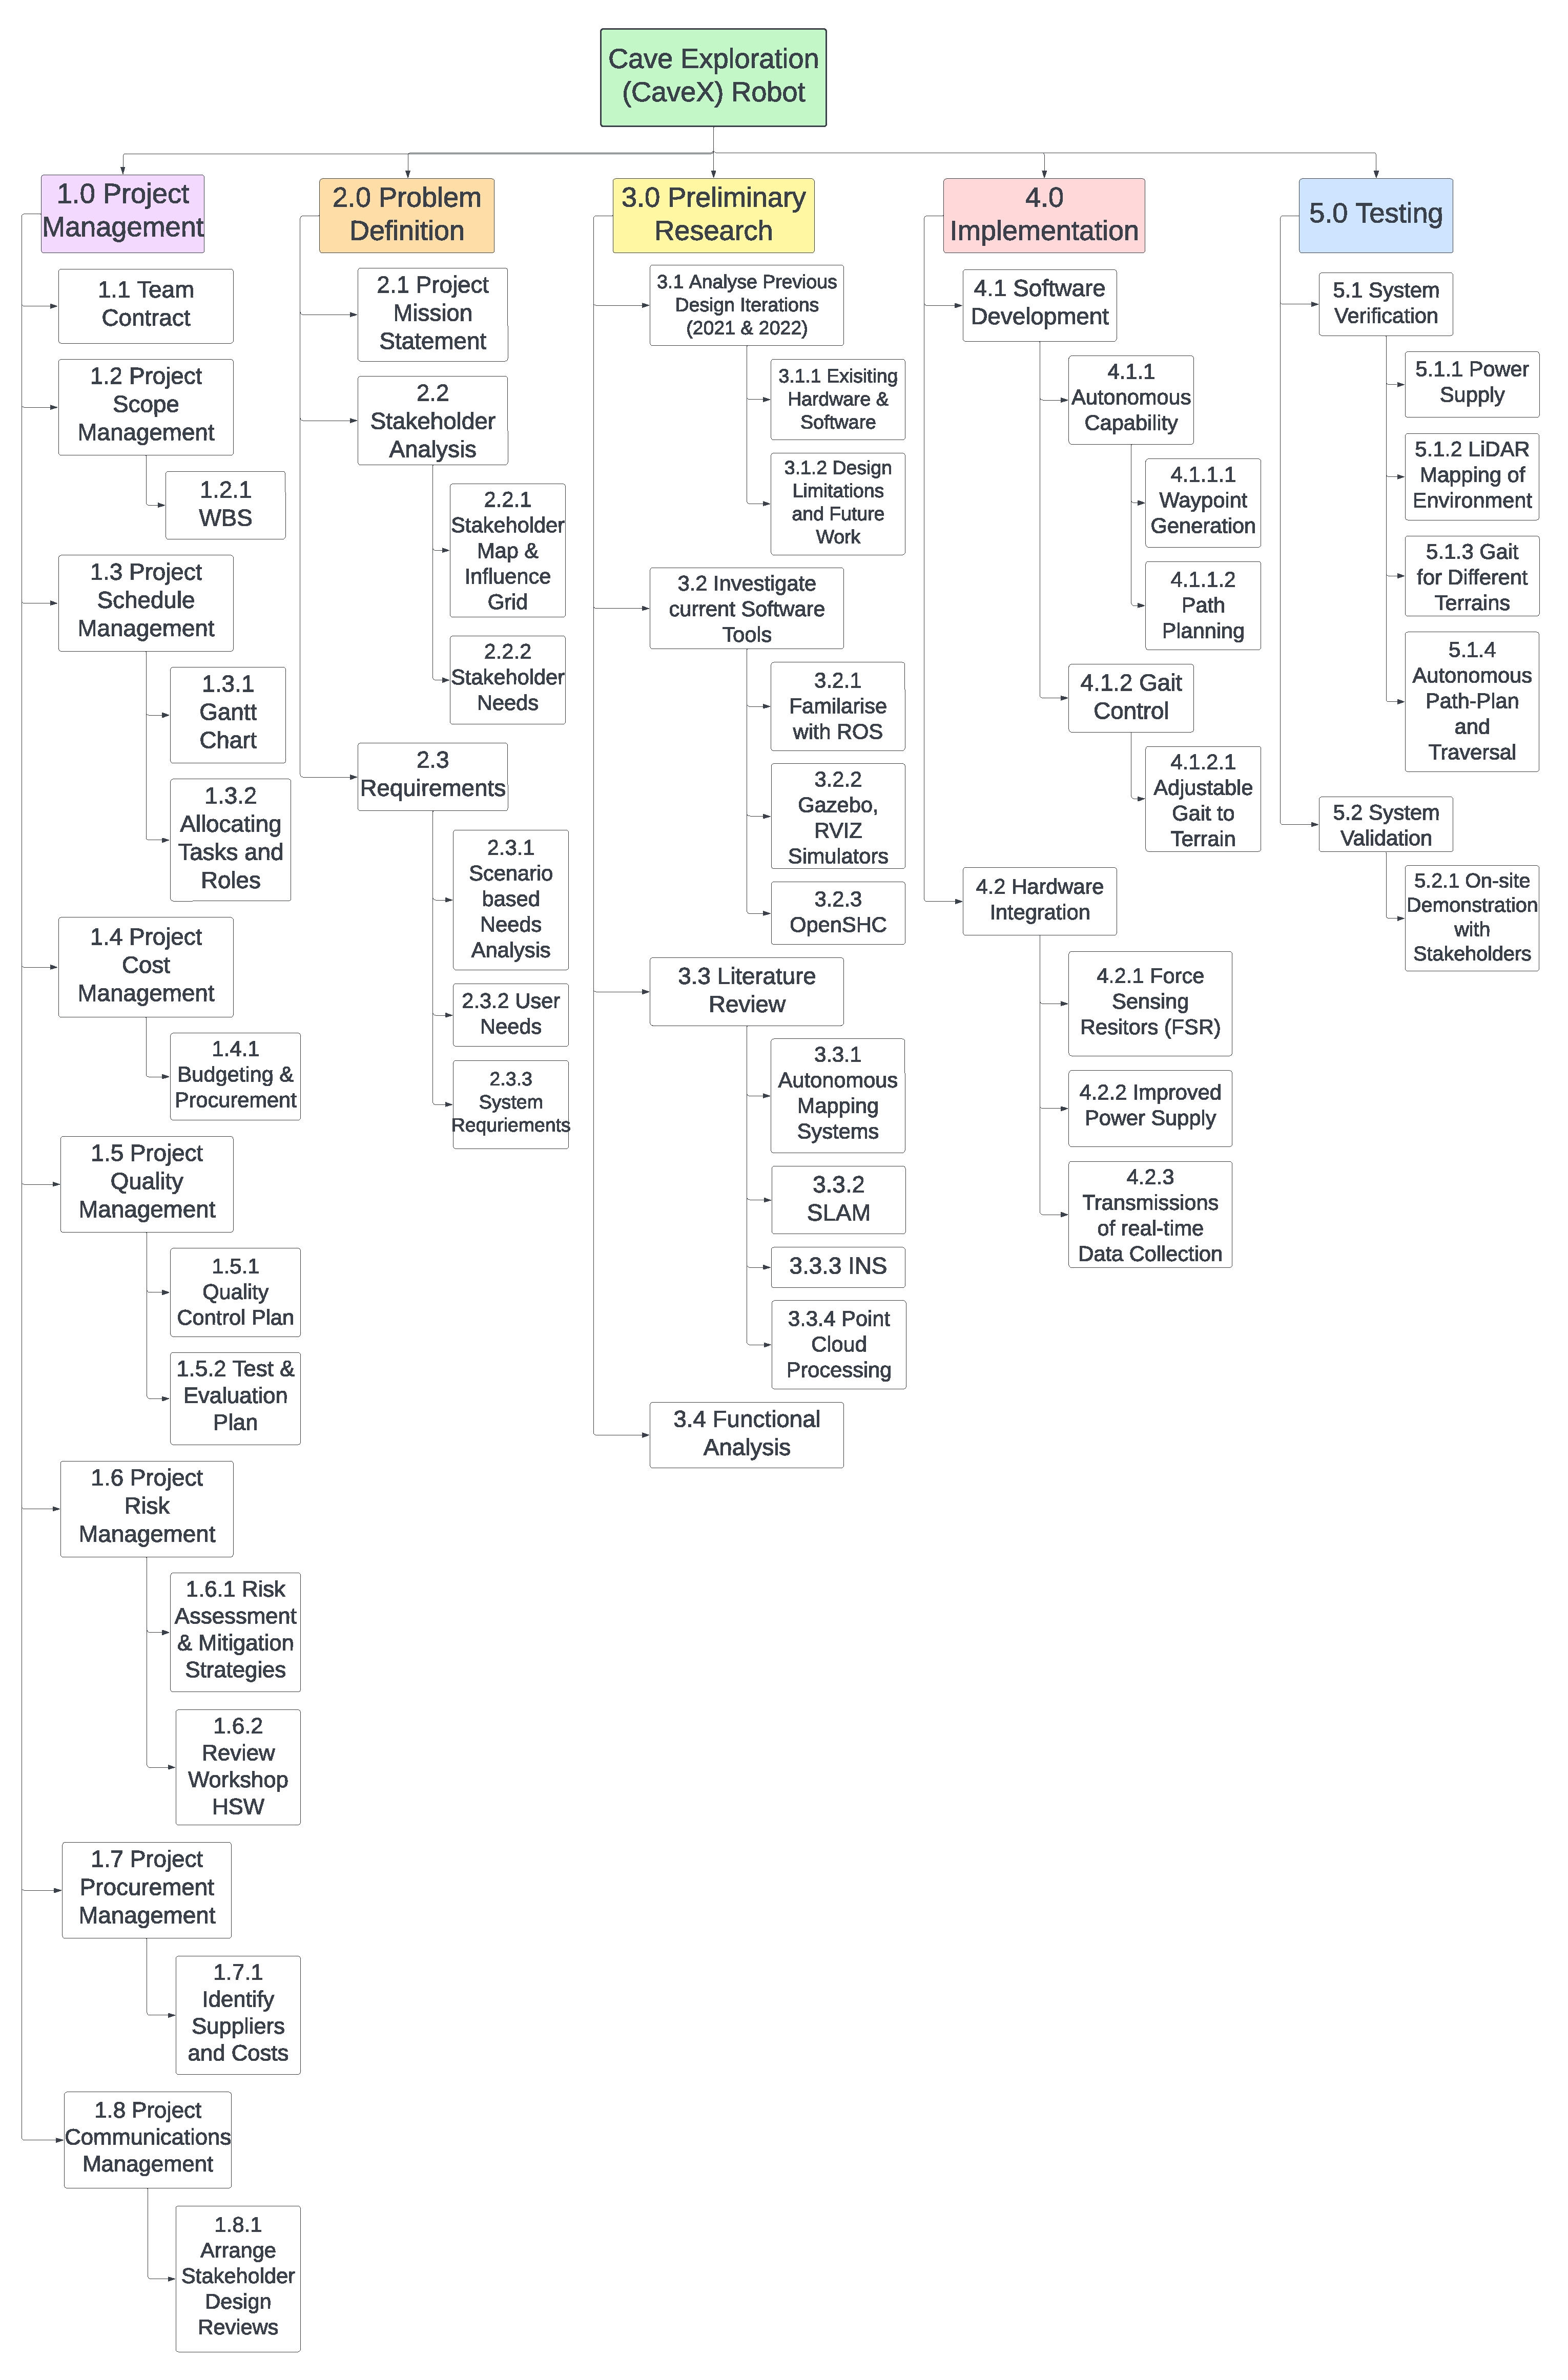
\includegraphics[page = 1, width = 0.95\textwidth]{WBS.pdf}

\newpage
\subsection{Gantt Chart}
\label{app:ganttChart}

\includegraphics[page = 1, width = 1.45\textwidth, angle = 90]{CaveX_2023_GanttChart_V3.0.pdf}

\includegraphics[page = 2, width = 1.45\textwidth, angle = 90]{CaveX_2023_GanttChart_V3.0.pdf}

\includegraphics[page = 3, width = 1.45\textwidth, angle = 90]{CaveX_2023_GanttChart_V3.0.pdf}

\newpage
\subsection{Sprint Plan}
\label{app:sprintplan}
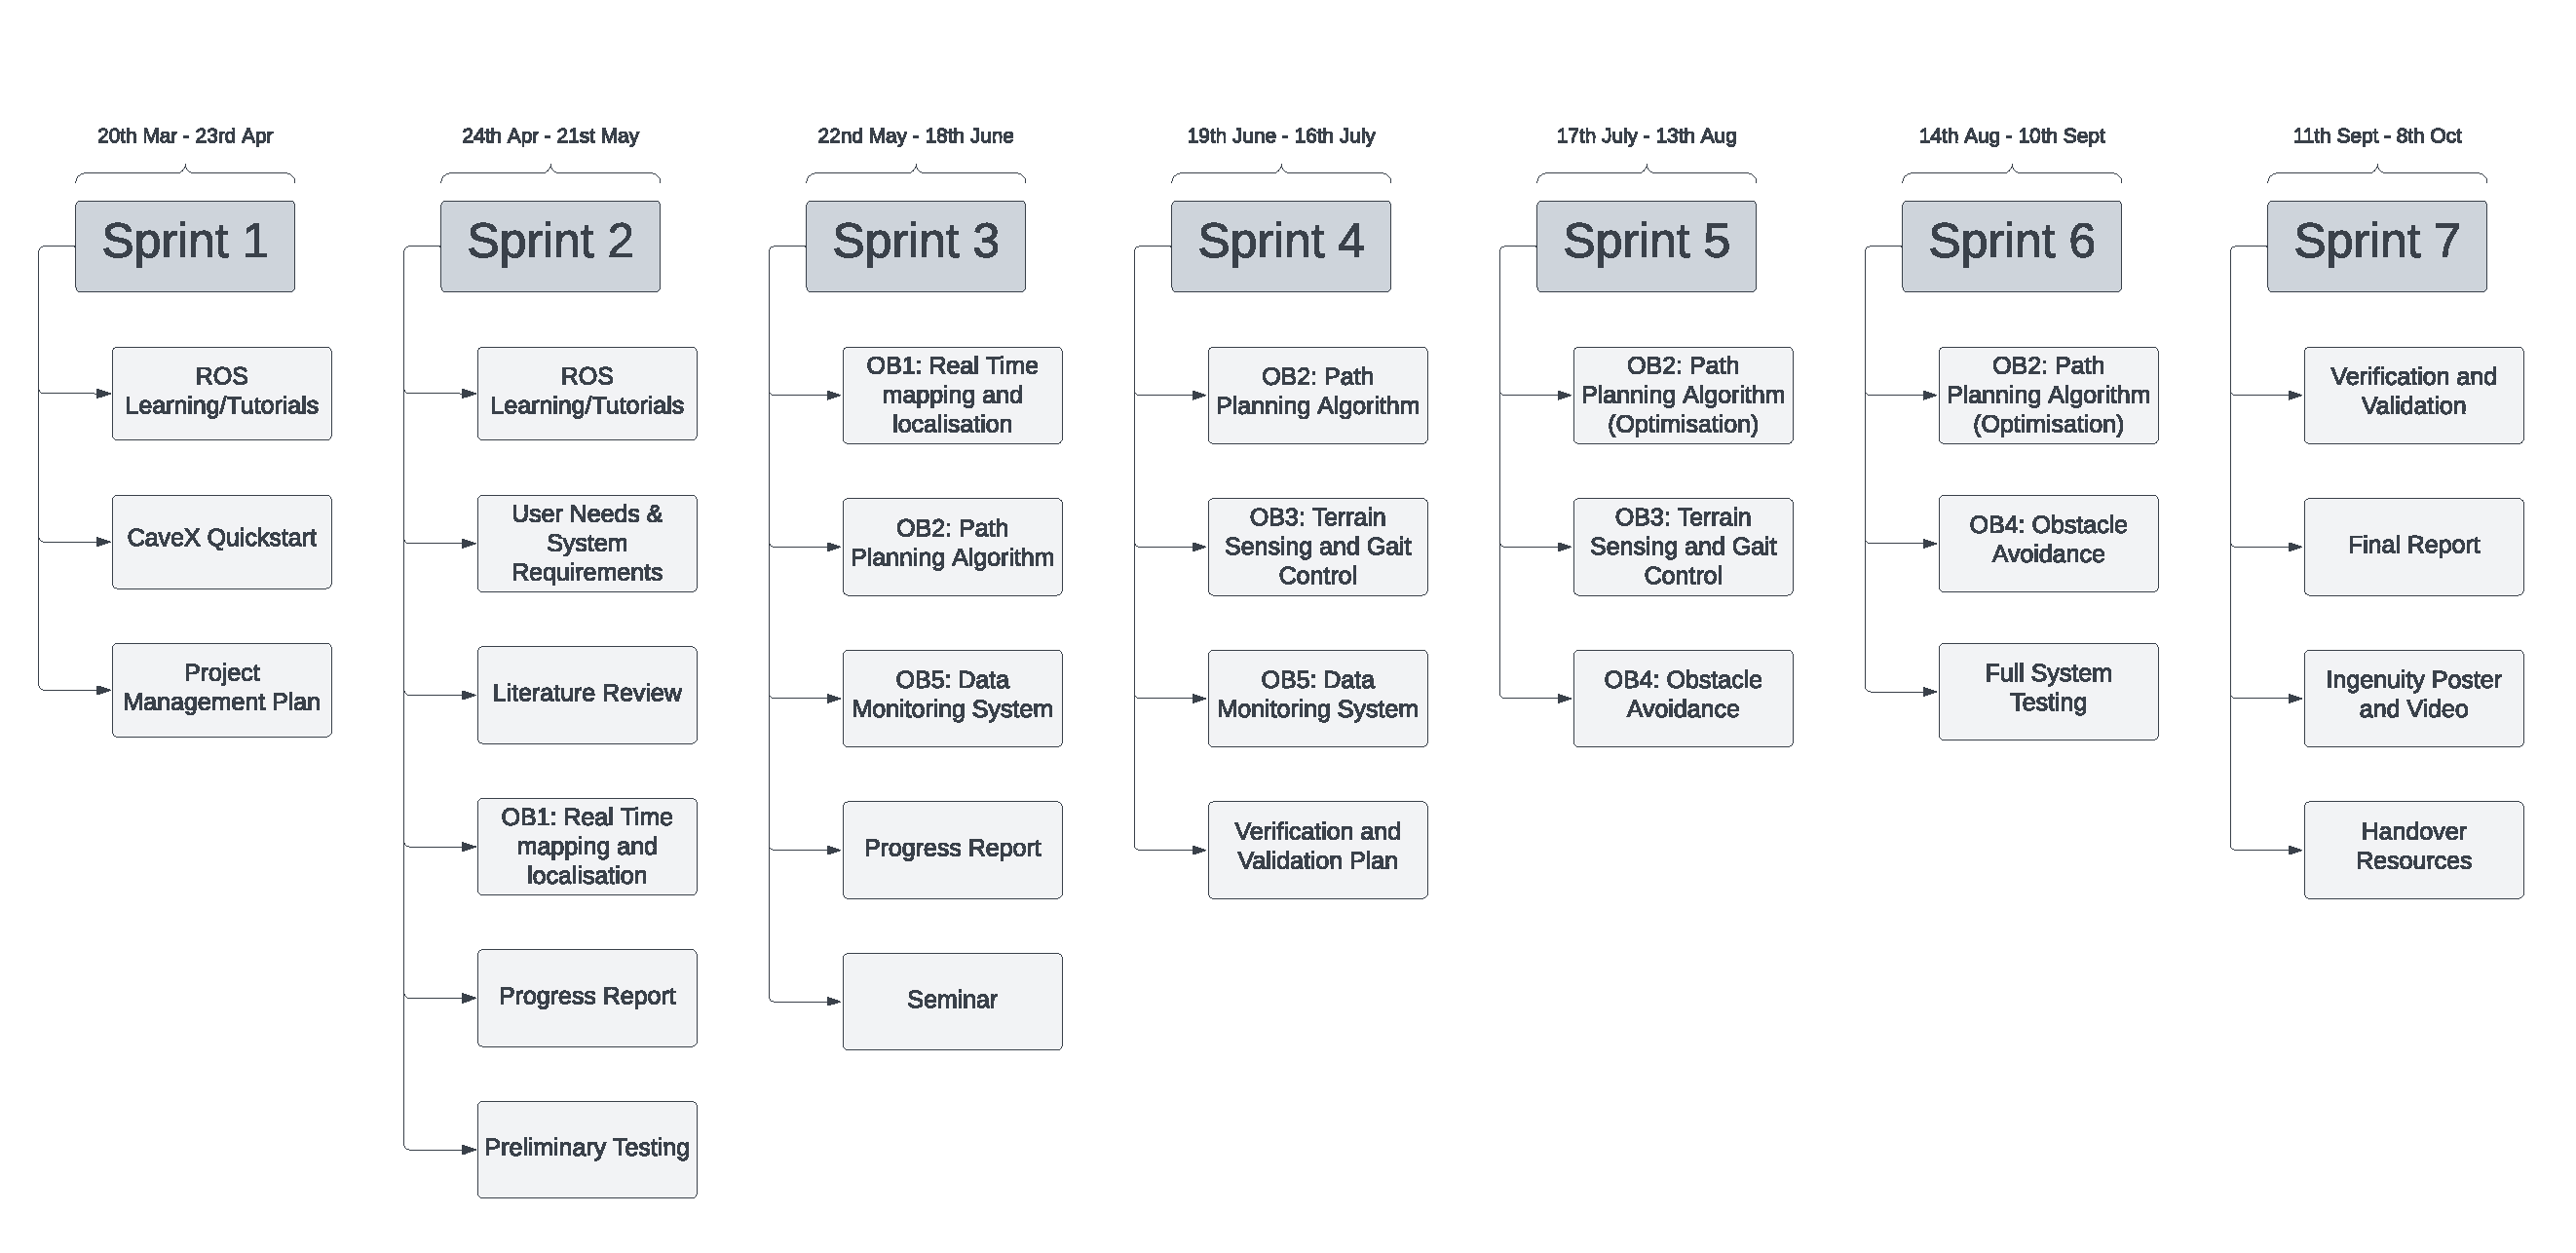
\includegraphics[page=1, scale=0.5, angle=90]{Sprint Plan.pdf}

\newpage
\subsection{Risk and Safety}
\label{app:riskmanagement}
Two types of risks, project risks and safety risks, were assessed to minimise the chance of negative outcomes throughout the project. Project risks are those which could impact the progress of the project as a whole. Safety risks are those which could adversely effect the health of anyone involved in or in the vicinity of project operations.

\newpage
\begin{landscape}
\subsubsection{Project Risks}
\bgroup
\rowcolors{2}{white}{gray!25}
\begin{xltabular}{0.99\linewidth}{M{2.3cm}M{3cm}M{2cm}M{2.2cm}M{2cm}M{3.8cm}M{2cm}M{2cm}M{2cm}}
    \caption{Project risk assessment for CaveX 2023 Honours Project} \label{apptab:riskassess} \\
    \hline \rowcolor{gray!50}
    \textbf{\large Event Context:} & \multicolumn{8}{|c}{\textbf{\large CaveX 2023 Honours Project Plan}} \\
    \hline
    Identified Risk & Impact & Initial Likelihood & Initial Severity & Initial Risk & Mitigation Strategies & New Likelihood & New Severity & Residual Risk \\ \hline
    \csvreader[late after line = \\, separator = semicolon]{./csv/riskass.csv}{1 = \risk, 2 = \imp, 3 = \intli, 4 = \intse, 5 = \intri, 6 = \nms, 7 = \nli, 8 = \nse, 9 = \rr}{\risk & \imp & \licell{\intli} & \secell{\intse} & \ricell{\intri} & \nms & \licell{\nli} & \secell{\nse} & \ricell{\rr}}
    \hline
\end{xltabular}
\egroup
\end{landscape}

\newpage
\subsubsection{Safety Risks}
The key safety risks which have needed to be considered regard the safe operation of the robot and the incline testing rig in the EXTERRES laboratory. The Risk Assessment (RA) and Safe Operating Procedure (SOP) for the robot use and the incline testing rig is included in this appendix.

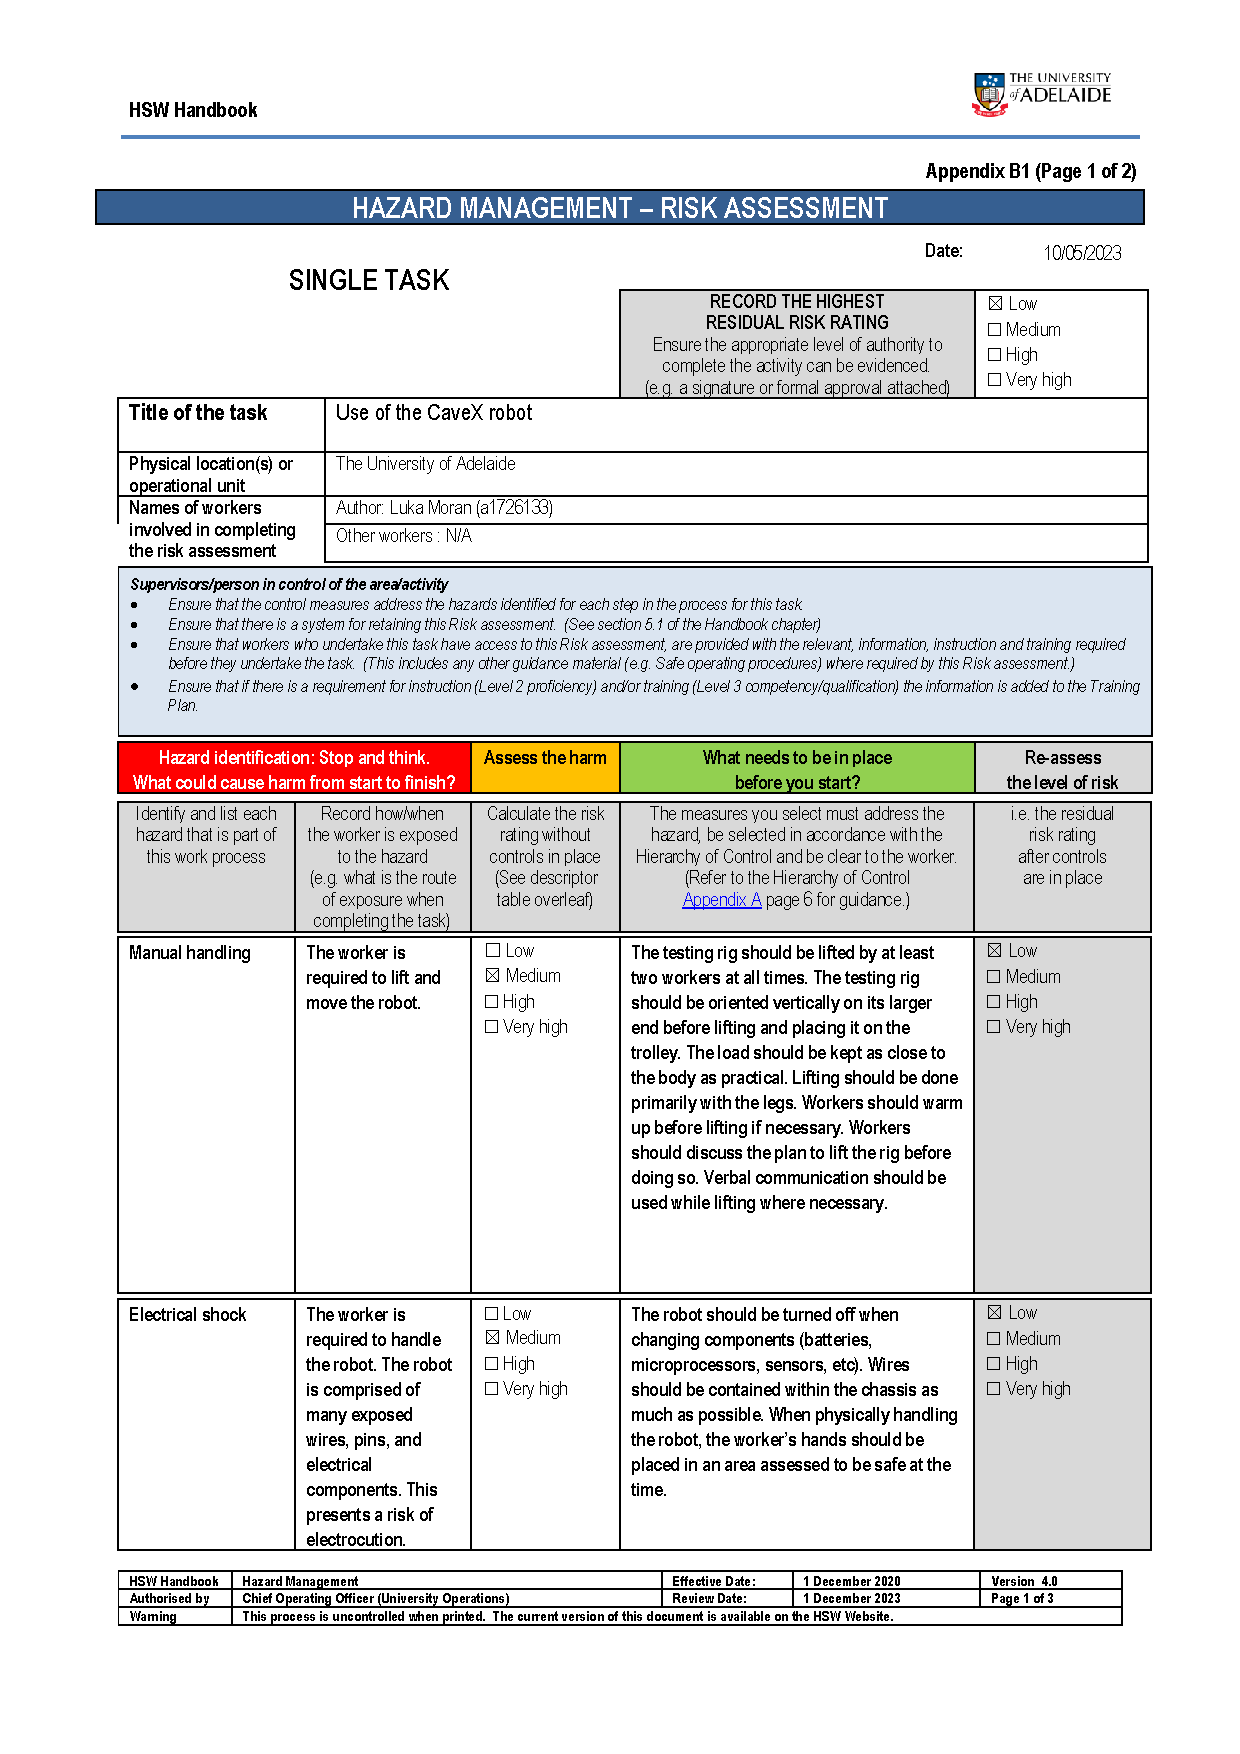
\includegraphics[page = 1, width = 0.9\textwidth]{RAs-SOPs/CaveX_RobotOperationRiskAssessment-Signed.pdf}

\includegraphics[page = 2, width = 0.9\textwidth]{RAs-SOPs/CaveX_RobotOperationRiskAssessment-Signed.pdf}

\includegraphics[page = 3, width = 0.9\textwidth]{RAs-SOPs/CaveX_RobotOperationRiskAssessment-Signed.pdf}

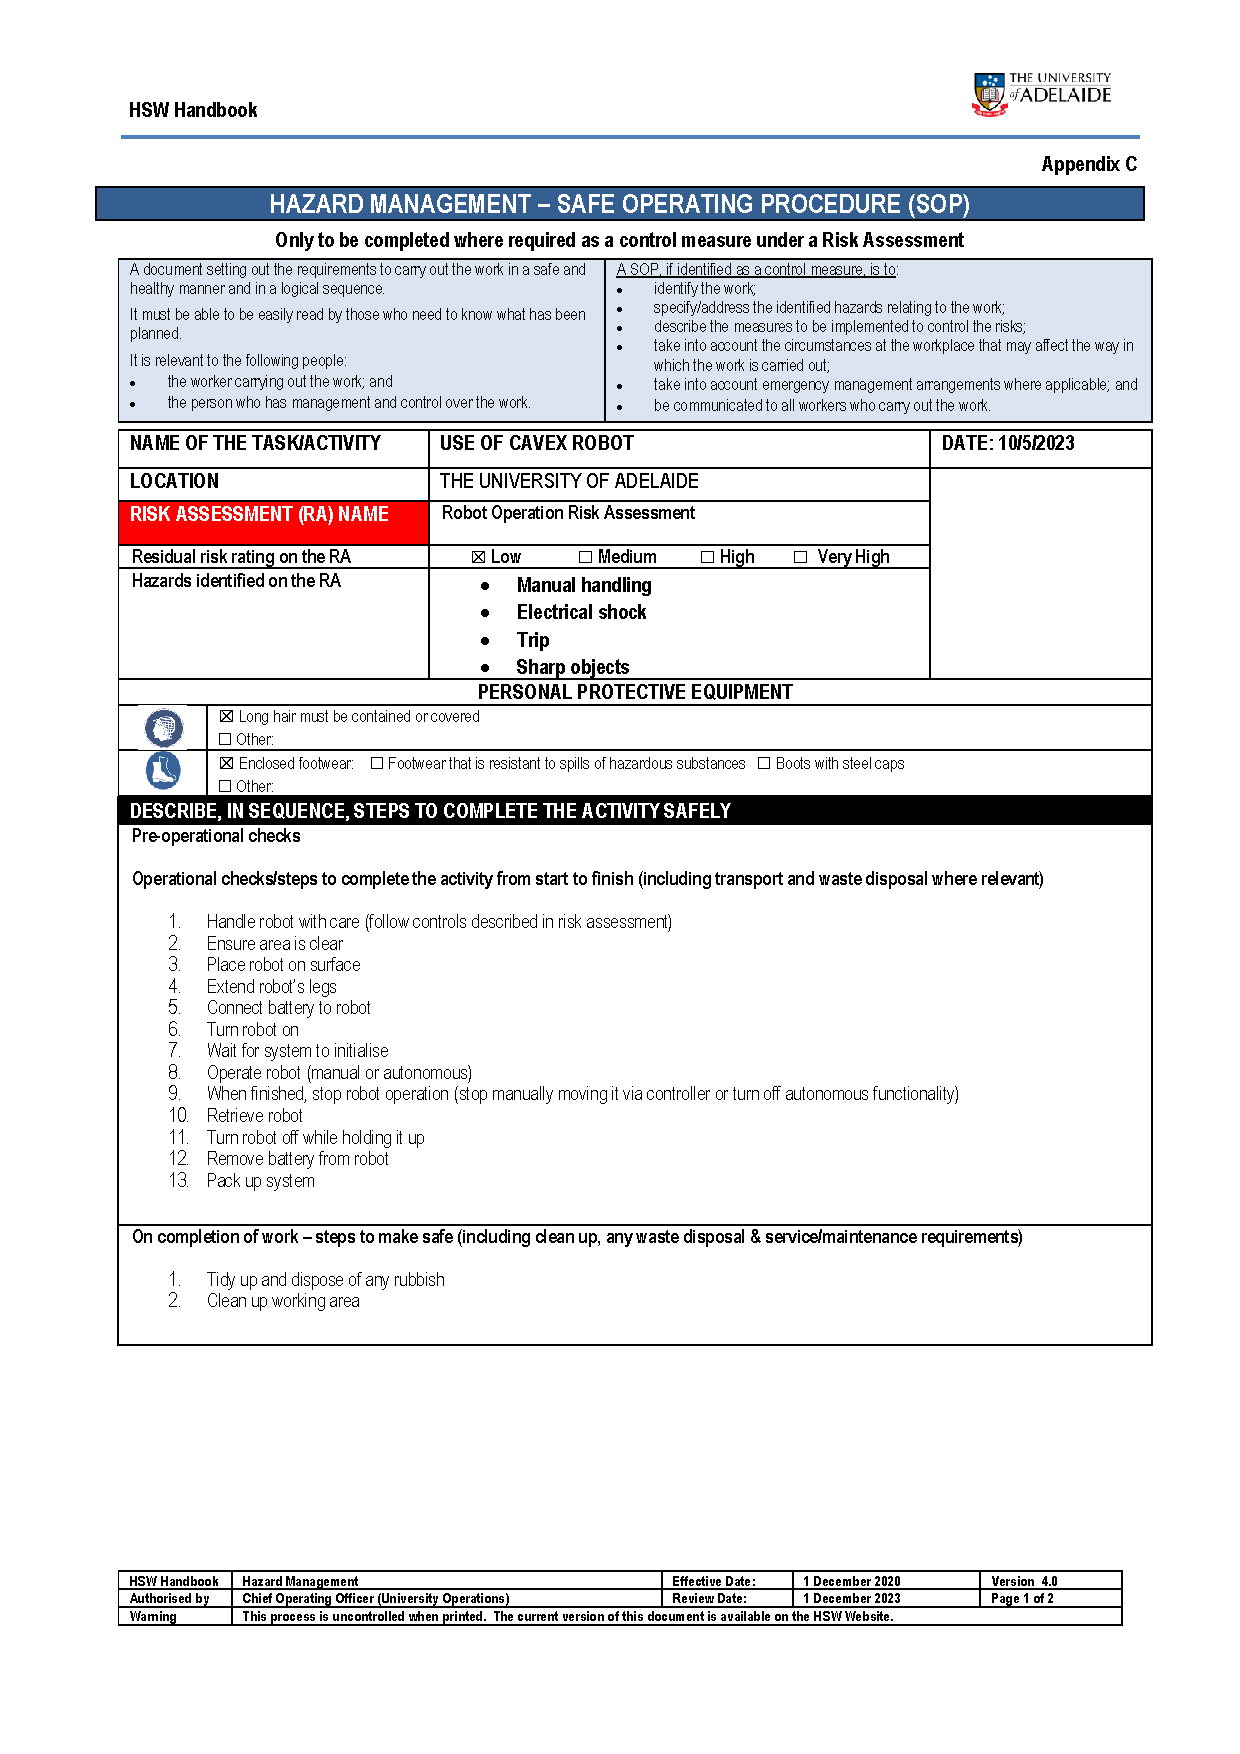
\includegraphics[page = 1, width = 0.9\textwidth]{RAs-SOPs/CaveX_RobotOperationSOP-Signed.pdf}

\includegraphics[page = 2, width = 0.9\textwidth]{RAs-SOPs/CaveX_RobotOperationSOP-Signed.pdf}

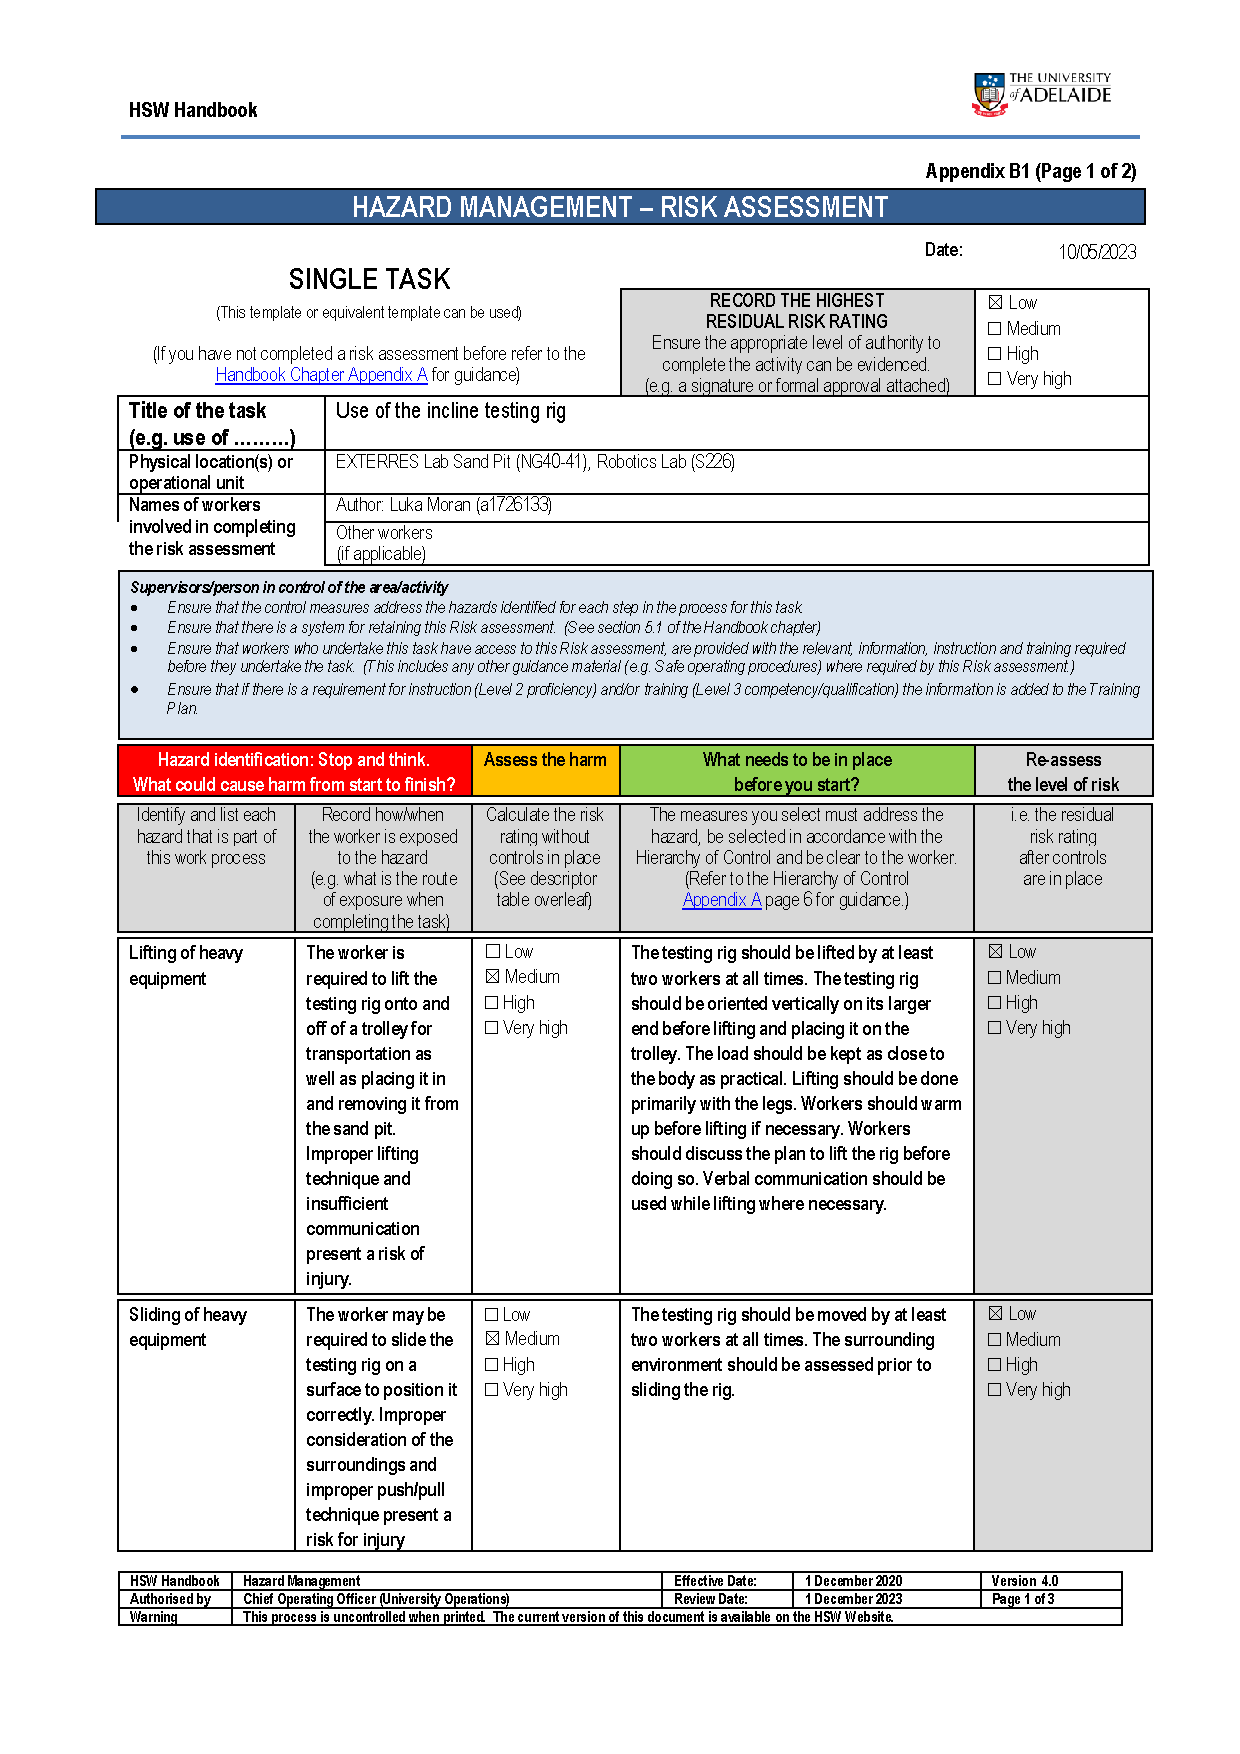
\includegraphics[page = 1, width = 0.9\textwidth]{RAs-SOPs/CaveX_InclineTestRigRiskAssessment-Signed.pdf}

\includegraphics[page = 2, width = 0.9\textwidth]{RAs-SOPs/CaveX_InclineTestRigRiskAssessment-Signed.pdf}

\includegraphics[page = 3, width = 0.9\textwidth]{RAs-SOPs/CaveX_InclineTestRigRiskAssessment-Signed.pdf}

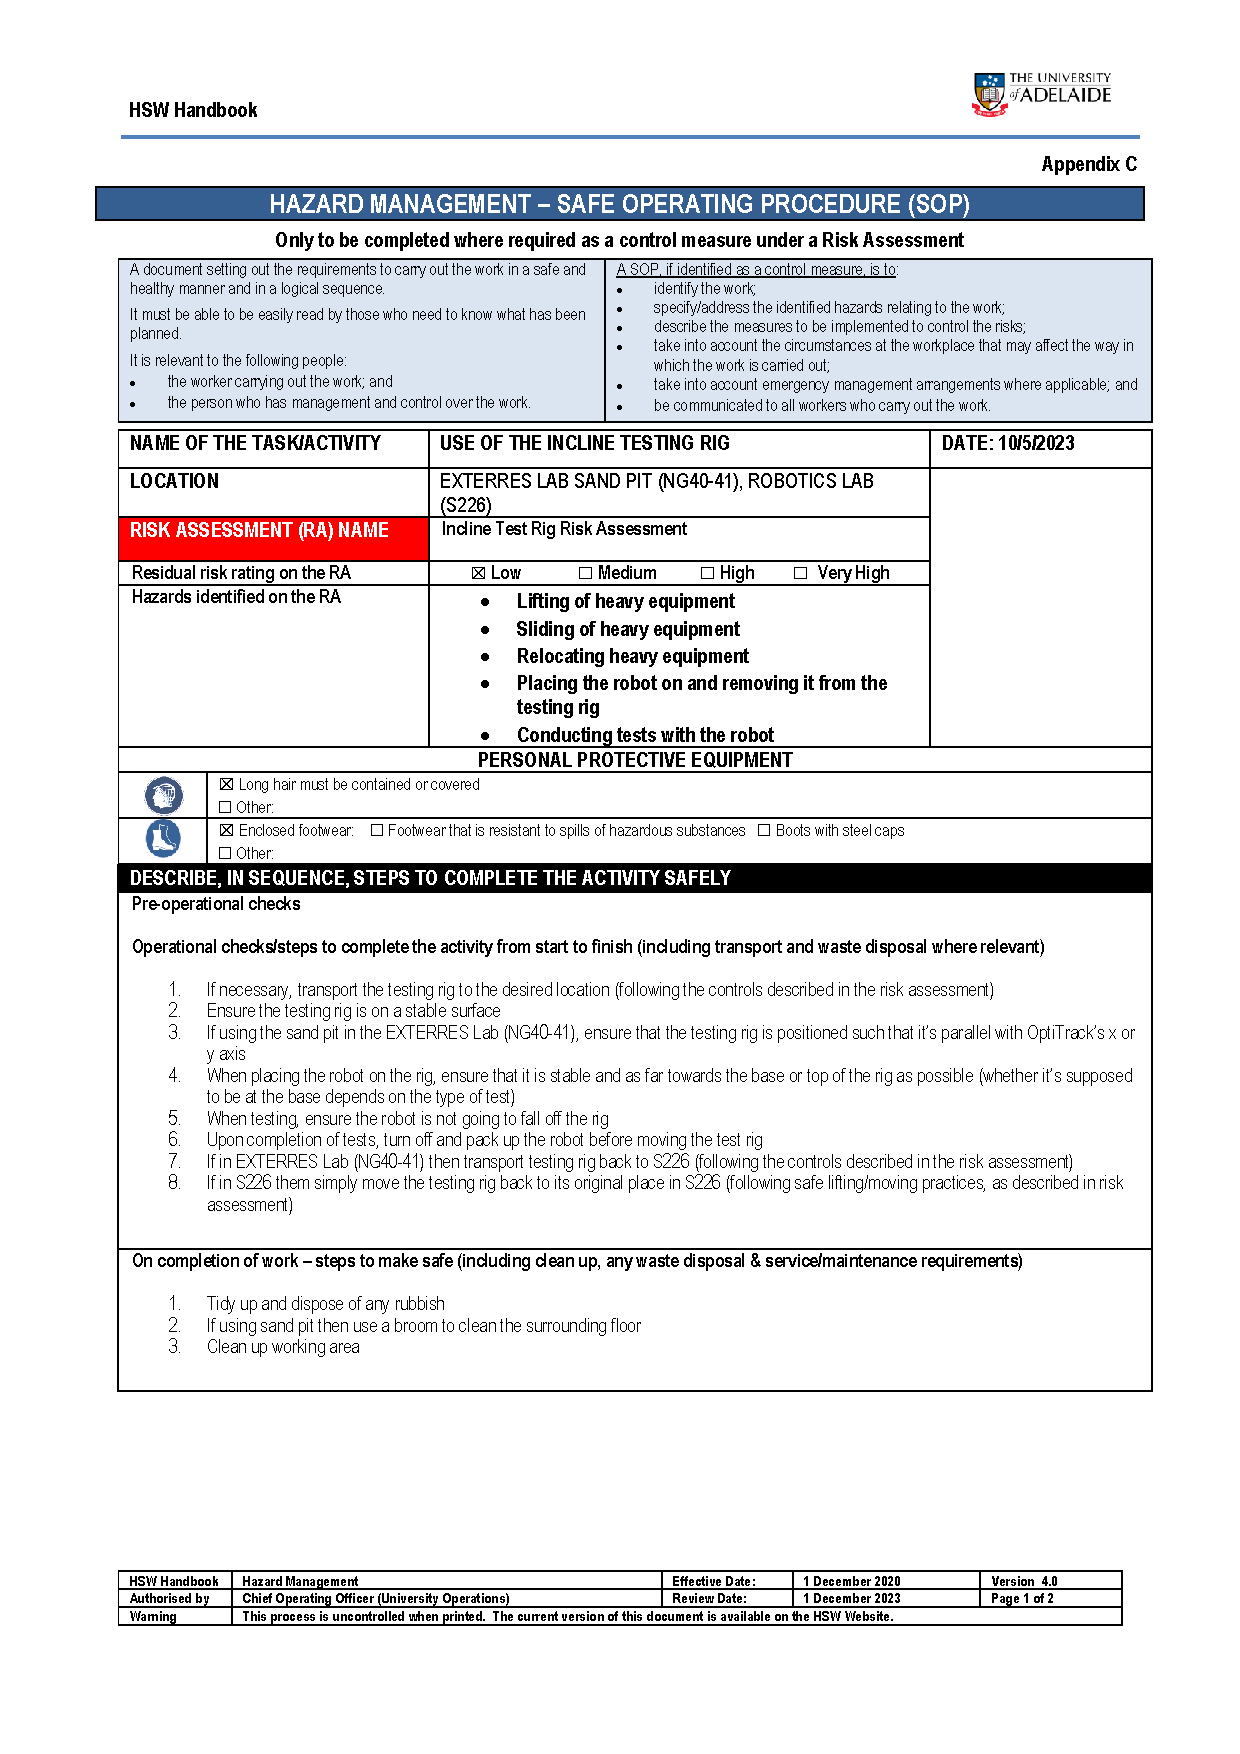
\includegraphics[page = 1, width = 0.9\textwidth]{RAs-SOPs/CaveX_InclineTestRigSOP-Signed.pdf}

\includegraphics[page = 2, width = 0.9\textwidth]{RAs-SOPs/CaveX_InclineTestRigSOP-Signed.pdf}

\newpage
\subsection{Quality Management}
\label{app:qualityplan}


\includegraphics[page = 1, width = \textwidth]{CaveX_2023__Quality_Management.pdf}


\includegraphics[page = 2, width = \textwidth]{CaveX_2023__Quality_Management.pdf}


\includegraphics[page = 3, width = \textwidth]{CaveX_2023__Quality_Management.pdf}


\includegraphics[page = 4, width = \textwidth]{CaveX_2023__Quality_Management.pdf}


\includegraphics[page = 5, width = \textwidth]{CaveX_2023__Quality_Management.pdf}